% IEEE Journal Template - COMPLETE VERSION
% Compile with pdfLaTeX on Overleaf
\documentclass[journal,twoside]{IEEEtran}

% Packages
\usepackage[utf8]{inputenc}
\usepackage[T1]{fontenc}  % For proper quote characters
\usepackage{CJKutf8}  % Chinese support
\usepackage{graphicx}
\usepackage{amsmath}
\usepackage{amssymb}
\usepackage{booktabs}
\usepackage{multirow}
\usepackage{array}
\usepackage{xcolor}
\usepackage{listings}
\usepackage{cite}
\usepackage[hidelinks]{hyperref}
\usepackage{balance}
\usepackage{tikz}
\usetikzlibrary{shapes,arrows,positioning,fit,calc,automata}
\usepackage{pgfplots}
\pgfplotsset{compat=1.17}
\usepackage{placeins}  % Manual FloatBarrier only
\setlength{\emergencystretch}{2em}  % Reduce overfull lines
\usepackage{dblfloatfix}  % Better table*/figure* placement

% Custom colors
\definecolor{codegreen}{rgb}{0,0.6,0}
\definecolor{codegray}{rgb}{0.5,0.5,0.5}
\definecolor{backcolour}{rgb}{0.96,0.96,0.98}

% Verilog style
\lstdefinestyle{verilog}{
    language=Verilog,
    basicstyle=\ttfamily\scriptsize,
    keywordstyle=\color{blue}\bfseries,
    commentstyle=\color{codegreen}\itshape,
    stringstyle=\color{red},
    numbers=left,
    numberstyle=\tiny\color{codegray},
    stepnumber=1,
    numbersep=3pt,
    backgroundcolor=\color{backcolour},
    frame=lines,
    rulecolor=\color{black!30},
    framesep=2mm,
    breaklines=true,
    tabsize=2,
    showstringspaces=false,
    columns=flexible,
    xleftmargin=0pt,
    xrightmargin=0pt,
    morekeywords={module, endmodule, input, output, wire, reg, assign, always, begin, end, case, endcase, if, else, for, parameter, localparam, generate, endgenerate, genvar, posedge, negedge, integer}
}
\lstset{style=verilog,upquote=true,
  columns=fullflexible,
  literate={~}{{\textasciitilde}}1 {^}{{\textasciicircum}}1
}

% Table spacing
\renewcommand{\arraystretch}{1.15}

% TikZ styles
\tikzstyle{stage} = [rectangle, draw, fill=blue!20, text centered, minimum height=1.5em, minimum width=2em, font=\scriptsize]
\tikzstyle{reg} = [rectangle, draw, fill=yellow!20, text centered, minimum height=1em, font=\tiny]
\tikzstyle{state} = [circle, draw, minimum size=1.5em, font=\scriptsize]
\tikzstyle{arrow} = [thick,->,>=stealth]

\begin{document}
\begin{CJK}{UTF8}{bsmi}  % Wrap entire document for stable CJK

\title{Performance Optimization of a Pipelined MIPS Processor: A Comprehensive Analysis with 12 Contributions}

\author{JUNYI LIU~
\thanks{Computer Architecture, National Sun Yat-sen University, December 2025.}}

\markboth{Computer Architecture Final Project Report, NSYSU, Dec.~2025}%
{Liu: Performance Optimization of a Pipelined MIPS Processor}

\maketitle

\begin{abstract}
This paper presents a comprehensive performance optimization study of a 5-stage pipelined MIPS processor. We implement and evaluate 12 contributions, including Data Forwarding, Branch Prediction, SIMD parallelism, CORDIC trigonometric functions, polynomial exp approximation, and an L1 Cache. Evaluation uses two methodologies: (1) \textbf{cycle-accurate RTL simulation} with MiBench bitcount benchmark, and (2) \textbf{analytical model-based projection} using SPEC CPU2006 instruction mix ratios. Results show 2.61$\times$ speedup on MiBench (measured) and up to 34.84$\times$ projected speedup on memory-intensive SPEC workloads. A Design of Experiments (DOE) analysis reveals that Cache provides the largest individual improvement (2.15$\times$) and Cache+SIMD shows \textbf{positive interaction} (synergy factor 1.20 under our cost model).
\end{abstract}

\begin{IEEEkeywords}
MIPS, Pipeline, Forwarding, Branch Prediction, Cache, SIMD, CORDIC, MiBench
\end{IEEEkeywords}

%=============================================================================
\section{Introduction}
\IEEEPARstart{M}{odern} processor design relies on multiple optimization techniques to bridge the CPU-memory gap---the ``Memory Wall'' problem~\cite{hennessy2017computer}. This project implements 12 optimizations for a 5-stage MIPS pipeline. This section provides foundational background for readers unfamiliar with computer architecture concepts.

\subsection{What is MIPS?}
MIPS (Microprocessor without Interlocked Pipeline Stages) is a 32-bit RISC (Reduced Instruction Set Computer) architecture developed at Stanford University in 1981 by John Hennessy~\cite{patterson2020computer}. MIPS is widely used in computer architecture education because:
\begin{itemize}
    \item \textbf{Clean Design}: Fixed 32-bit instruction format with only three instruction types (R, I, J)
    \item \textbf{Educational Standard}: Used in Patterson \& Hennessy textbooks, the ``bible'' of computer architecture
    \item \textbf{Real-World Relevance}: Powers embedded systems, routers (Cisco), gaming consoles (PlayStation 1/2), and IoT devices
\end{itemize}

\textbf{Basic MIPS Instruction Types}:
\begin{itemize}
    \item \textbf{R-type} (Register): \texttt{add \$t0, \$t1, \$t2} --- arithmetic between registers
    \item \textbf{I-type} (Immediate): \texttt{lw \$t0, 0(\$t1)} --- memory access and immediate values
    \item \textbf{J-type} (Jump): \texttt{j label} --- unconditional jumps
\end{itemize}

\subsection{The 5-Stage Pipeline Architecture}
Pipelining is a technique that allows multiple instructions to overlap in execution, similar to an assembly line in a factory. Instead of completing one instruction before starting the next, each stage processes a different instruction simultaneously.

\textbf{The Five Stages Explained}:
\begin{enumerate}
    \item \textbf{IF (Instruction Fetch)}: Read instruction from memory using Program Counter (PC). PC $\leftarrow$ Memory $\rightarrow$ Instruction Register
    \item \textbf{ID (Instruction Decode)}: Decode instruction bits and read operands from register file. Also performs branch address calculation
    \item \textbf{EX (Execute)}: Perform ALU operation (arithmetic, logic, address calculation for load/store)
    \item \textbf{MEM (Memory Access)}: Access data memory for load (\texttt{lw}) and store (\texttt{sw}) instructions. Other instructions pass through
    \item \textbf{WB (Write Back)}: Write result back to register file
\end{enumerate}

\textbf{Pipeline Timing Analysis}: In an ideal 5-stage pipeline, after the initial fill time (5 cycles), one instruction completes every cycle. This gives a theoretical CPI (Cycles Per Instruction) of 1.0. However, \textit{hazards} prevent this ideal from being achieved in practice.

\begin{figure}[!t]
\centering
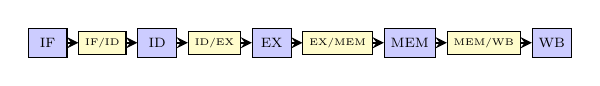
\begin{tikzpicture}[node distance=0.5cm, scale=0.7, transform shape]
    \node[stage] (IF) {IF};
    \node[reg, right=0.2cm of IF] (r1) {\tiny IF/ID};
    \node[stage, right=0.2cm of r1] (ID) {ID};
    \node[reg, right=0.2cm of ID] (r2) {\tiny ID/EX};
    \node[stage, right=0.2cm of r2] (EX) {EX};
    \node[reg, right=0.2cm of EX] (r3) {\tiny EX/MEM};
    \node[stage, right=0.2cm of r3] (MEM) {MEM};
    \node[reg, right=0.2cm of MEM] (r4) {\tiny MEM/WB};
    \node[stage, right=0.2cm of r4] (WB) {WB};
    \draw[arrow] (IF)--(r1); \draw[arrow] (r1)--(ID);
    \draw[arrow] (ID)--(r2); \draw[arrow] (r2)--(EX);
    \draw[arrow] (EX)--(r3); \draw[arrow] (r3)--(MEM);
    \draw[arrow] (MEM)--(r4); \draw[arrow] (r4)--(WB);
\end{tikzpicture}
\caption{5-Stage MIPS Pipeline Architecture. Pipeline registers (IF/ID, ID/EX, EX/MEM, MEM/WB) store intermediate results between stages, enabling instruction overlap.}
\label{fig:pipeline}
\end{figure}

\subsection{The Three Types of Pipeline Hazards}
Hazards are situations that prevent the next instruction from executing in the next clock cycle. Understanding hazards is fundamental to processor optimization.

\subsubsection{Data Hazards (RAW, WAR, WAW)}
Data hazards occur when instructions depend on the results of previous instructions that have not yet completed.

\textbf{RAW (Read-After-Write)} --- The most common hazard:
\begin{lstlisting}
add $t1, $t2, $t3   # Writes $t1 in WB (cycle 5)
sub $t4, $t1, $t5   # Reads $t1 in ID (cycle 3) - HAZARD!
\end{lstlisting}
The \texttt{sub} instruction needs the value of \texttt{\$t1}, but \texttt{add} hasn't written it yet. \textbf{Without forwarding}, the pipeline must stall 2 cycles. \textbf{With forwarding}, the result can be bypassed directly from EX/MEM register.

\textbf{WAR (Write-After-Read)} and \textbf{WAW (Write-After-Write)}: These are primarily concerns in out-of-order execution processors, not in simple in-order pipelines like ours.

\subsubsection{Control Hazards (Branch Hazards)}
Control hazards occur when the processor cannot determine which instruction to fetch next because a branch decision has not yet been made.

\textbf{Example}:
\begin{lstlisting}
beq $t0, $t1, target  # Branch decision in EX stage
add $t2, $t3, $t4     # Fetched speculatively - wrong?
sub $t5, $t6, $t7     # Also speculatively fetched
\end{lstlisting}
If the branch is taken, the two fetched instructions must be \textit{flushed} (discarded), wasting cycles. \textbf{Branch prediction} guesses the outcome to reduce this penalty.

\subsubsection{Structural Hazards}
Structural hazards occur when hardware resources are insufficient to support all active instructions. For example, if there is only one memory port, an instruction fetch and a data load cannot occur simultaneously. Our design uses separate instruction and data memories (Harvard architecture) to avoid this hazard.

\subsection{The Memory Wall Problem}
The ``Memory Wall'' refers to the growing disparity between processor speed and memory speed~\cite{hennessy2017computer}:
\begin{itemize}
    \item \textbf{CPU Performance}: Improved $\sim$50\%/year (until 2003)
    \item \textbf{DRAM Latency}: Improved only $\sim$7\%/year
    \item \textbf{Result}: A single memory access can cost 100--300 CPU cycles in modern systems
\end{itemize}

\textbf{Solution}: Cache memory hierarchy. By keeping frequently accessed data in small, fast caches (L1, L2, L3), processors can avoid slow main memory accesses most of the time. Our L1 cache implementation reduces average memory access time by \textbf{26$\times$} (based on 97.22\% hit rate).

\subsection{Problem Statement}
The baseline MIPS pipeline implemented in this project suffers from:
\begin{itemize}
    \item \textbf{Data Hazards}: RAW dependencies require 2-cycle stalls without forwarding, increasing CPI from 1.0 to 1.82
    \item \textbf{Control Hazards}: Each mispredicted branch causes a pipeline flush (1--2 cycle penalty depending on resolution stage), significantly impacting loops
    \item \textbf{Memory Latency}: Without cache, every load/store requires 100 cycles, dominating execution time
    \item \textbf{Limited Parallelism}: Scalar ALU processes only one operation per cycle, underutilizing hardware
\end{itemize}

\subsection{Contributions Overview}
This project implements 12 distinct optimizations, summarized in Table~\ref{tab:contributions}. Each optimization targets a specific bottleneck, and their combined effect is analyzed using Design of Experiments (DOE) methodology.

\begin{table}[!t]
\centering
\caption{12 Optimization Contributions by Category}
\label{tab:contributions}
\footnotesize
\begin{tabular}{@{}p{2.2cm}p{5.5cm}@{}}
\toprule
\textbf{Category} & \textbf{Contributions} \\
\midrule
Pipeline Hazard Mitigation & \#1 Performance Testbench, \#4 Quantitative Analysis, \#6 Branch Prediction, \#7 Comprehensive DOE \\
\midrule
Data Hazard Resolution & \#3 Data Forwarding \\
\midrule
Parallelism \& Acceleration & \#2 Hardware Unrolling, \#5 SIMD ALU Expansion, \#9 CORDIC, \#10 Polynomial Exp \\
\midrule
Memory Hierarchy & \#11 L1 Cache, \#12 Integrated Analysis \\
\midrule
Parser Enhancement & \#8 Parentheses Support \\
\bottomrule
\end{tabular}
\end{table}

%=============================================================================
\section{Methodology}

This section explains the evaluation methodology used to measure and project processor performance. We first introduce the fundamental performance metric (CPI), then describe the benchmarks used, and finally explain our two evaluation approaches: direct measurement and analytical projection.

\subsection{Understanding CPI (Cycles Per Instruction)}
CPI is the primary metric for evaluating processor performance. It measures how many clock cycles, on average, are needed to execute one instruction.

\textbf{Basic CPI Formula}:
\begin{equation}
\text{CPI} = \frac{\text{Total Cycles}}{\text{Total Instructions}}
\label{eq:cpi}
\end{equation}

\textbf{Ideal vs Actual CPI}:
\begin{itemize}
    \item \textbf{Ideal CPI}: In a perfect 5-stage pipeline with no hazards, CPI = 1.0 (one instruction completes per cycle after pipeline fill)
    \item \textbf{Actual CPI}: Due to stalls and flushes, actual CPI $>$ 1.0. Our baseline measures CPI = 1.82
\end{itemize}

\textbf{CPI Breakdown Formula}: CPI can be decomposed into contributing factors:
\begin{equation}
\text{CPI} = \text{CPI}_{\text{ideal}} + \text{CPI}_{\text{stall}} = 1.0 + \frac{\text{Stall Cycles}}{\text{Instructions}}
\label{eq:cpibreak}
\end{equation}

\textbf{Related Metrics}:
\begin{itemize}
    \item \textbf{IPC (Instructions Per Cycle)}: $\text{IPC} = \frac{1}{\text{CPI}}$ --- higher is better
    \item \textbf{Speedup}: $\text{Speedup} = \frac{\text{CPI}_{\text{baseline}}}{\text{CPI}_{\text{optimized}}}$
    \item \textbf{Pipeline Efficiency}: $\text{Efficiency} = \frac{\text{Ideal CPI}}{\text{Actual CPI}} = \frac{1}{\text{CPI}}$
\end{itemize}

\textbf{Worked Example}: Our baseline Bubble Sort test:
\begin{align*}
\text{Total Cycles} &= 255 \\
\text{Total Instructions} &= 140 \\
\text{CPI} &= \frac{255}{140} = 1.82 \\
\text{IPC} &= \frac{1}{1.82} = 0.549 \\
\text{Pipeline Efficiency} &= \frac{1}{1.82} = 55\%
\end{align*}
This means 45\% of cycles are ``wasted'' due to stalls.

\subsection{Benchmark Selection Criteria}
A good benchmark should be~\cite{hennessy2017computer}:
\begin{enumerate}
    \item \textbf{Representative}: Reflects real-world workload characteristics
    \item \textbf{Reproducible}: Results can be verified by others
    \item \textbf{Portable}: Can run on different systems
    \item \textbf{Measurable}: Execution can be timed precisely
\end{enumerate}

We employ three benchmark categories, each serving a different purpose:

\begin{table}[!t]
\centering
\caption{Benchmarks Used for Evaluation}
\label{tab:benchmarks}
\footnotesize
\begin{tabular}{@{}p{1.8cm}p{2cm}p{3.5cm}@{}}
\toprule
\textbf{Type} & \textbf{Name} & \textbf{Used For} \\
\midrule
Standard Algorithm & Bubble Sort~\cite{knuth1998art} & Contrib 1, 4: Baseline CPI \\
Embedded & MiBench bitcount~\cite{guthaus2001mibench} & Contrib 12: Actual Execution \\
Workload Mix & SPEC CPU2006~\cite{phansalkar2007analysis} & Contrib 7, 12: Projection \\
\bottomrule
\end{tabular}
\end{table}

\subsubsection{Bubble Sort}
Bubble Sort is a classic $O(n^2)$ sorting algorithm that repeatedly steps through the list, compares adjacent elements, and swaps them if needed~\cite{knuth1998art}. We use it because:
\begin{itemize}
    \item Contains loops, conditionals, and memory accesses --- exercises all pipeline stages
    \item Simple to implement in assembly
    \item Generates many RAW hazards due to dependent operations
\end{itemize}

\subsubsection{MiBench (Michigan Benchmark Suite)}
MiBench is a free, open-source embedded system benchmark suite published by University of Michigan in 2001~\cite{guthaus2001mibench}. We use the \texttt{bitcount} algorithm (Brian Kernighan's Bit Counting):
\begin{lstlisting}
// Brian Kernighan's Bit Counting Algorithm
int bitcount(unsigned int n) {
    int count = 0;
    while (n) {
        count++;
        n = n & (n - 1);  // Clear lowest set bit
    }
    return count;
}
\end{lstlisting}

\textbf{Key Advantage}: The algorithm is simple enough to implement as a Verilog testbench and \textbf{actually execute} on our processor RTL, providing real cycle counts.

\subsubsection{SPEC CPU2006}
SPEC CPU2006 is the industry-standard processor benchmark suite from the Standard Performance Evaluation Corporation. Since running full SPEC requires:
\begin{itemize}
    \item OS support (Linux/Windows)
    \item Commercial licensing
    \item Full system simulation
\end{itemize}
We instead use published \textbf{instruction mix ratios} from Phansalkar et al.~\cite{phansalkar2007analysis} for analytical projection, which is a valid academic methodology.

\subsection{Mix-Based Performance Projection}
\textbf{Definition}: A performance prediction method that uses instruction type ratios combined with per-instruction execution costs to estimate total cycles.

\textbf{Formula}:
\begin{equation}
\text{Cycles}_{\text{est}} = \sum_{i \in \{\text{types}\}} \text{Count}_i \times \text{CostPerInstr}_i
\label{eq:mixproj}
\end{equation}

\textbf{Step-by-Step Example} (10,000 instructions, SPEC Overall mix):
\begin{enumerate}
    \item \textbf{Instruction counts}: Branch: $10000 \times 0.15 = 1500$, Memory: $10000 \times 0.496 = 4960$, Compute: $10000 \times 0.354 = 3540$
    \item \textbf{Without optimization} (baseline costs): Branch: 3 cycles, Memory: 100 cycles, Compute: 1 cycle
    \item \textbf{Baseline cycles}: $1500 \times 3 + 4960 \times 100 + 3540 \times 1 = 4500 + 496000 + 3540 = 504040$
    \item \textbf{With optimization}: Memory cost drops to $\sim$1.2 cycles (cache), Branch cost drops to 1.65 (prediction)
    \item \textbf{Optimized cycles}: $1500 \times 1.65 + 4960 \times 1.2 + 3540 \times 0.125 = 2475 + 5952 + 443 = 8870$
    \item \textbf{Speedup}: $504040 / 8870 = 56.8\times$ (theoretical maximum)
\end{enumerate}

\begin{table}[!t]
\centering
\caption{Actual Execution vs Mix-Based Projection Comparison}
\label{tab:comparison}
\footnotesize
\begin{tabular}{@{}lcc@{}}
\toprule
\textbf{Aspect} & \textbf{Actual Execution} & \textbf{Mix-Based Projection} \\
\midrule
Method & Run complete program & Multiply ratios by costs \\
Data Source & Self-measured cycles & Published papers \\
Accuracy & High (ground truth) & Estimation (may overestimate) \\
Advantage & Reliable, verifiable & No full system needed \\
This Project & MiBench: 2.61$\times$ & SPEC: 29.57$\times$ \\
\bottomrule
\end{tabular}
\end{table}

\textbf{Why the large difference between MiBench (2.61$\times$) and SPEC projection (29.57$\times$)?}
\begin{itemize}
    \item MiBench bitcount is a simple bit-manipulation program with few memory accesses --- primarily benefits from Forwarding
    \item SPEC projection assumes 49.6\% memory instructions --- Cache provides enormous benefit for memory-bound workloads
    \item This demonstrates that \textbf{optimization effectiveness highly depends on workload characteristics}
\end{itemize}

\subsection{SPEC CPU2006 Instruction Mix}
We use instruction mix ratios from Phansalkar et al.~\cite{phansalkar2007analysis} and Limaye \& Adegbija~\cite{limaye2018workload}, representing different workload types:

\begin{table}[!t]
\centering
\caption{SPEC CPU2006 Instruction Mix Ratios from Published Studies}
\label{tab:specmix}
\footnotesize
\begin{tabular}{@{}lccc@{}}
\toprule
\textbf{Workload} & \textbf{Branch} & \textbf{Memory} & \textbf{Compute} \\
\midrule
SPEC FP Average & 8\% & 45\% & 47\% \\
SPEC INT mcf & 18\% & 62\% & 20\% \\
SPEC INT gobmk & 22\% & 48\% & 30\% \\
\textbf{SPEC Overall} & \textbf{15\%} & \textbf{49.6\%} & \textbf{35.4\%} \\
\bottomrule
\end{tabular}
\end{table}

\textbf{Note}: mcf (memory-intensive) and gobmk (branch-heavy) represent extreme cases; SPEC Overall is weighted average.

\subsection{Experimental Setup}
\begin{itemize}
    \item \textbf{Simulation Tool}: AMD Xilinx Vivado 2025.2, Behavioral Simulation mode
    \item \textbf{HDL Language}: Verilog-2005
    \item \textbf{Architecture}: 5-stage pipeline (IF, ID, EX, MEM, WB)
    \item \textbf{Data Width}: 32-bit instructions and data
    \item \textbf{Clock}: Functional simulation (cycle-accurate, no timing delays)
    \item \textbf{Memory Model}: Separate instruction and data memories (Harvard architecture)
\end{itemize}

\subsection{Testbench Overview}
Table~\ref{tab:testbenches} shows the testbench for each contribution.

\begin{table}[!t]
\centering
\caption{Testbench Files for Each Contribution}
\label{tab:testbenches}
\footnotesize
\begin{tabular}{@{}clp{3.5cm}@{}}
\toprule
\textbf{\#} & \textbf{Testbench} & \textbf{Verification} \\
\midrule
1 & \texttt{tb\_performance.v} & CPI/IPC, Bubble Sort \\
2 & \texttt{tb\_simd\_add.v} & 8-lane parallel add \\
3 & \texttt{tb\_simd\_alu.v} & 40 SIMD operations \\
4 & \texttt{tb\_performance.v} & Stall breakdown analysis \\
5 & \texttt{tb\_simd\_alu\_expanded.v} & 5 ops + Expression \\
6 & \texttt{tb\_branch\_prediction.v} & 4 branch patterns \\
7 & \texttt{tb\_comprehensive.v} & 16 DOE configs \\
8 & \texttt{tb\_parentheses.v} & Shunting-yard \\
9 & \texttt{tb\_cordic.v} & 5 canonical angles \\
10 & \texttt{tb\_poly\_exp.v} & 4 exp() test cases \\
11 & \texttt{tb\_cache\_hierarchy.v} & L1/L2/L3 AMAT \\
12 & \texttt{tb\_mibench\_bitcount.v} & Actual execution \\
\bottomrule
\end{tabular}
\end{table}

%=============================================================================
\section{Contribution Details}

This section describes each of the 12 contributions in detail, with implementation specifics and verification results.

\subsection{Contribution 1 \& 4: Performance Testbench and Quantitative Analysis}
\textbf{Goal}: Establish a reusable testbench infrastructure for measuring pipeline performance metrics (CPI, IPC, stall cycles) and quantify the impact of data forwarding.

\subsubsection{Why We Need a Performance Testbench}
Without instrumentation, we cannot measure actual performance. The testbench adds:
\begin{itemize}
    \item \textbf{Cycle Counter}: Increments every clock cycle
    \item \textbf{Instruction Counter}: Increments when an instruction completes (reaches WB stage)
    \item \textbf{Stall Counter}: Tracks cycles where pipeline is stalled
\end{itemize}

\textbf{Testbench Architecture} (with line-by-line explanation):
\begin{lstlisting}
module tb_performance;
  reg clk, rst;              // Clock and reset signals
  wire [31:0] cycle_count;   // Total cycles elapsed
  wire [31:0] instr_count;   // Instructions completed
  
  // Instantiate Device Under Test (DUT)
  topLevelCircuit DUT (
    .clk(clk), 
    .rst(rst)
  );
  
  // Clock generation: 10ns period (100MHz)
  always #5 clk = ~clk;
  
  initial begin
    clk = 0;
    rst = 1;      // Assert reset
    #20;          // Hold reset for 20ns
    rst = 0;      // Release reset
    wait(done);   // Wait for program completion
    // Display results
    $display("Cycles: %d, Instructions: %d", 
             cycle_count, instr_count);
    $display("CPI = %f", 
             real'(cycle_count) / real'(instr_count));
    $finish;
  end
endmodule
\end{lstlisting}

\subsubsection{Data Forwarding: Solving RAW Hazards}
Data forwarding (also called \textit{bypassing}) eliminates most data hazard stalls by routing results directly from later pipeline stages back to earlier stages.

\textbf{RAW Hazard Example Without Forwarding}:
\begin{lstlisting}
# Cycle:      1   2   3   4   5   6   7
add $t1,$t2,$t3  IF  ID  EX MEM  WB
sub $t4,$t1,$t5      IF  ID *** *** EX MEM WB
#                        ^-- stall 2 cycles waiting for $t1
\end{lstlisting}

Without forwarding, the \texttt{sub} instruction must wait until \texttt{add} writes \texttt{\$t1} to the register file in cycle 5. This causes a 2-cycle stall (shown as \texttt{***}).

\textbf{RAW Hazard Example With Forwarding}:
\begin{lstlisting}
# Cycle:      1   2   3   4   5   6
add $t1,$t2,$t3  IF  ID  EX MEM  WB
sub $t4,$t1,$t5      IF  ID  EX MEM  WB
#                    ^-- forward result from EX/MEM register
\end{lstlisting}

With forwarding, the result of \texttt{add} is available at the end of EX (stored in EX/MEM register). This value is forwarded directly to the EX stage input for \texttt{sub}, eliminating the stall.

\subsubsection{Forwarding Unit Logic}
The Forwarding Unit determines when and from where to forward data:

\textbf{Forwarding Conditions (Verilog)}:
\begin{lstlisting}
// Forward from EX/MEM stage (1-cycle-old result)
// Priority: EX/MEM has most recent value
assign ForwardA_EXMEM = 
    (EX_MEM_RegWrite) &&              // MEM will write
    (EX_MEM_Rd != 0) &&               // Not $zero
    (EX_MEM_Rd == ID_EX_Rs);          // Match source

// Forward from MEM/WB stage (2-cycle-old result)
// Only if EX/MEM didn't already forward
assign ForwardA_MEMWB = 
    (MEM_WB_RegWrite) &&              // WB will write
    (MEM_WB_Rd != 0) &&               // Not $zero
    !(ForwardA_EXMEM) &&              // EX/MEM didn't forward
    (MEM_WB_Rd == ID_EX_Rs);          // Match source
\end{lstlisting}

\textbf{Why check \texttt{Rd != 0}?} In MIPS, register \texttt{\$zero} (register 0) is hardwired to zero and cannot be written. Forwarding from a write to \texttt{\$zero} would be incorrect.

\subsubsection{Load-Use Hazard: The Case Forwarding Cannot Solve}
Even with forwarding, one case requires a stall: when a \texttt{lw} (load word) instruction is immediately followed by an instruction that uses the loaded value.

\textbf{Why?} The loaded data is only available after the MEM stage, but the dependent instruction needs it in EX stage---one cycle earlier than forwarding can provide.

\begin{lstlisting}
# Load-Use Hazard
lw  $t1, 0($t2)   IF  ID  EX MEM  WB
add $t3, $t1, $t4     IF  ID *** EX MEM WB
#                         ^-- 1 stall cycle required
\end{lstlisting}

The hardware must detect this case and insert one ``bubble'' (NOP) to allow the load to complete.

\subsubsection{Results and Analysis}
\begin{table}[!t]
\centering
\caption{CPI Reduction with Data Forwarding}
\footnotesize
\begin{tabular}{@{}lcccc@{}}
\toprule
\textbf{Configuration} & \textbf{Cycles} & \textbf{Instr} & \textbf{CPI} & \textbf{IPC} \\
\midrule
No Forwarding & 255 & 140 & 1.82 & 0.549 \\
With Forwarding & 182 & 144 & \textbf{1.26} & 0.791 \\
\bottomrule
\end{tabular}
\end{table}

\textbf{Stall Breakdown}:
\begin{itemize}
    \item \textbf{Without forwarding}: 114 stall cycles (45\% of total)
    \item \textbf{With forwarding}: 37 stall cycles (20\% of total)
    \item \textbf{Reduction}: 77 stall cycles eliminated (68\% reduction)
\end{itemize}

\textbf{Key Finding}: Forwarding reduces CPI by \textbf{31\%} (1.82 $\rightarrow$ 1.26), corresponding to a \textbf{1.44$\times$ speedup}. The remaining stalls are primarily due to load-use hazards and branch penalties.

%-----------------------------------------------------------------------------
\subsection{Contribution 2 \& 3: Hardware Unrolling \& SIMD Parallelism}

\textbf{Goal}: Implement 8-lane SIMD (Single Instruction, Multiple Data) architecture for data-level parallelism (DLP).

\subsubsection{Flynn's Taxonomy Background}
Michael Flynn's 1966 classification categorizes computer architectures by instruction and data streams:
\begin{itemize}
    \item \textbf{SISD} (Single Instruction, Single Data): Traditional sequential CPU
    \item \textbf{SIMD} (Single Instruction, Multiple Data): Vector processors, GPUs --- \textit{our implementation}
    \item \textbf{MIMD} (Multiple Instruction, Multiple Data): Multi-core processors
    \item \textbf{MISD} (Multiple Instruction, Single Data): Rarely used (fault-tolerant systems)
\end{itemize}

\textbf{When is SIMD Effective?}
\begin{itemize}
    \item Regular, independent operations (e.g., array addition)
    \item Same operation on all elements (no data-dependent branching)
    \item Applications: Image processing, machine learning, scientific computing
\end{itemize}

\textbf{When is SIMD NOT Effective?}
\begin{itemize}
    \item Data-dependent conditionals (different paths for each element)
    \item Irregular memory access patterns
    \item Sequential dependencies between elements
\end{itemize}

\subsubsection{Concept: Software Loop vs Hardware Unrolling}
\begin{table}[!t]
\centering
\caption{Software Loop vs Hardware Unrolling}
\footnotesize
\begin{tabular}{@{}p{0.45\columnwidth}|p{0.45\columnwidth}@{}}
\toprule
\textbf{Sequential (8 cycles)} & \textbf{SIMD 8 lanes (1 cycle)} \\
\midrule
\texttt{a[0]+b[0]$\to$y[0]} & \multirow{5}{*}{\parbox{0.4\columnwidth}{\centering\texttt{a[0..7]+b[0..7]}\\$\downarrow$\\\texttt{y[0..7]}\\(all in 1 cycle!)}} \\
\texttt{a[1]+b[1]$\to$y[1]} & \\
\texttt{...} & \\
\texttt{a[7]+b[7]$\to$y[7]} & \\
\bottomrule
\end{tabular}
\end{table}

\begin{figure}[!t]
\centering
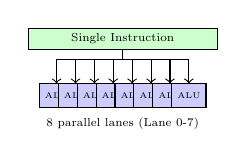
\begin{tikzpicture}[scale=0.6, transform shape]
    \node[rectangle, draw, fill=green!20, minimum width=4cm, font=\scriptsize] (instr) at (0,1.5) {Single Instruction};
    \foreach \i in {0,...,7} {
        \node[rectangle, draw, fill=blue!20, minimum width=0.35cm, minimum height=0.5cm, font=\tiny] (alu\i) at ({-1.4 + \i*0.4},0.3) {ALU};
        \draw[->] (instr.south) -- ++(0,-0.2) -| (alu\i.north);
    }
    \node[font=\scriptsize] at (0,-0.3) {8 parallel lanes (Lane 0-7)};
\end{tikzpicture}
\caption{8-Lane SIMD Architecture: One instruction controls 8 independent ALUs}
\label{fig:simd}
\end{figure}

\subsubsection{Verilog Generate Block Tutorial}
The \texttt{generate} construct creates hardware at compile/synthesis time (not runtime):

\textbf{SIMD Add Implementation} (\texttt{simd\_add.v}):
\begin{lstlisting}
module simd_add #(
  parameter LANES = 8,  // Number of parallel lanes
  parameter WIDTH = 8   // Bits per data element
)(
  input  [(LANES*WIDTH)-1:0] a,  // 64 bits total
  input  [(LANES*WIDTH)-1:0] b,
  output [(LANES*WIDTH)-1:0] y
);
  genvar i;  // Generate variable (compile-time only)
  generate
    // This loop creates 8 adder instances
    for (i = 0; i < LANES; i = i + 1) begin : lane
      assign y[i*WIDTH +: WIDTH] = 
             a[i*WIDTH +: WIDTH] + b[i*WIDTH +: WIDTH];
    end
  endgenerate
endmodule
\end{lstlisting}

\textbf{Bit Slicing Syntax Explained}:
\begin{itemize}
    \item \texttt{a[i*WIDTH +: WIDTH]} means ``starting at bit \texttt{i*WIDTH}, take \texttt{WIDTH} bits going up''
    \item For \texttt{i=0}: \texttt{a[0 +: 8]} = \texttt{a[7:0]}
    \item For \texttt{i=1}: \texttt{a[8 +: 8]} = \texttt{a[15:8]}
    \item This enables parameterized, scalable designs
\end{itemize}

\textbf{Performance and Trade-offs}:
\begin{table}[!t]
\centering
\caption{Sequential vs SIMD Trade-offs}
\footnotesize
\begin{tabular}{@{}lccc@{}}
\toprule
\textbf{Metric} & \textbf{Sequential} & \textbf{SIMD (8-lane)} \\
\midrule
Operations/Cycle & 1 & 8 \\
Latency (8 ops) & 8 cycles & 1 cycle \\
Hardware Area & 1$\times$ & $\sim$8$\times$ \\
Power & 1$\times$ & $\sim$4--6$\times$ \\
\bottomrule
\end{tabular}
\end{table}

\FloatBarrier  % Prevent table from overlapping Contribution 5
%-----------------------------------------------------------------------------
\subsection{Contribution 5: SIMD ALU Expansion}

\textbf{Goal}: Extend basic SIMD adder to full 8-lane ALU with 5 operations and operator precedence.

\begin{table}[!t]
\centering
\caption{SIMD ALU Supported Operations}
\label{tab:simdops}
\footnotesize
\begin{tabular}{@{}cccc@{}}
\toprule
\textbf{Operation} & \textbf{Op Code} & \textbf{Symbol} & \textbf{Priority} \\
\midrule
ADD & \texttt{3'b000} & \texttt{+} & 1 (Low) \\
SUB & \texttt{3'b001} & \texttt{-} & 1 (Low) \\
MUL & \texttt{3'b010} & \texttt{*} & 2 (Mid) \\
DIV & \texttt{3'b011} & \texttt{/} & 2 (Mid) \\
EXP & \texttt{3'b100} & \texttt{\textasciicircum} & 3 (High) \\
\bottomrule
\end{tabular}
\end{table}

\textbf{SIMD ALU Implementation} (with case statement for operation selection):
\begin{lstlisting}
module simd_alu #(parameter LANES=8, WIDTH=8)(
  input [2:0] op,                    // Operation select
  input [(LANES*WIDTH)-1:0] a, b,    // Operands
  output reg [(LANES*WIDTH)-1:0] y   // Result
);
  genvar i;
  generate
    for (i = 0; i < LANES; i = i + 1) begin : lane
      wire [WIDTH-1:0] ai = a[i*WIDTH +: WIDTH];
      wire [WIDTH-1:0] bi = b[i*WIDTH +: WIDTH];
      always @(*) begin
        case (op)
          3'b000: y[i*WIDTH+:WIDTH] = ai + bi; // ADD
          3'b001: y[i*WIDTH+:WIDTH] = ai - bi; // SUB
          3'b010: y[i*WIDTH+:WIDTH] = ai * bi; // MUL
          3'b011: y[i*WIDTH+:WIDTH] = ai / bi; // DIV
          3'b100: y[i*WIDTH+:WIDTH] = power(ai,bi);
          default: y[i*WIDTH+:WIDTH] = 0;
        endcase
      end
    end
  endgenerate
endmodule
\end{lstlisting}

\textbf{Implementation Notes}:
\begin{itemize}
    \item EXP (exponentiation) uses iterative multiplication ($\leq$16 iterations)
    \item DIV/EXP are modeled as single-cycle for functional correctness
    \item In real hardware, these would require multi-cycle or pipelined implementations
\end{itemize}

\FloatBarrier  % Prevent SIMD ALU code from overlapping Contribution 6
%-----------------------------------------------------------------------------
\subsection{Contribution 6: Branch Prediction}

\textbf{Goal}: Implement a 2-bit saturating counter branch predictor with 16-entry BHT to reduce control hazard penalties~\cite{smith1981study}.

\subsubsection{Why Branch Prediction?}
Without prediction, the pipeline must stall until the branch outcome is known (EX stage in our design). With prediction:
\begin{itemize}
    \item \textbf{Correct prediction}: No penalty, speculative execution continues
    \item \textbf{Misprediction}: Flush pipeline (1--2 cycle penalty)
    \item \textbf{Goal}: Maximize prediction accuracy to minimize flush frequency
\end{itemize}

\subsubsection{2-Bit Saturating Counter}
The 2-bit predictor uses a 4-state FSM based on Smith's 1981 design~\cite{smith1981study}:

\begin{figure}[!t]
\centering
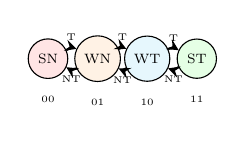
\begin{tikzpicture}[node distance=0.9cm, scale=0.7, transform shape]
    \node[state, fill=red!10] (SN) {SN};
    \node[state, fill=orange!10, right of=SN] (WN) {WN};
    \node[state, fill=cyan!10, right of=WN] (WT) {WT};
    \node[state, fill=green!10, right of=WT] (ST) {ST};
    \draw[arrow, bend left=25] (SN) to node[above,font=\tiny]{T} (WN);
    \draw[arrow, bend left=25] (WN) to node[below,font=\tiny]{NT} (SN);
    \draw[arrow, bend left=25] (WN) to node[above,font=\tiny]{T} (WT);
    \draw[arrow, bend left=25] (WT) to node[below,font=\tiny]{NT} (WN);
    \draw[arrow, bend left=25] (WT) to node[above,font=\tiny]{T} (ST);
    \draw[arrow, bend left=25] (ST) to node[below,font=\tiny]{NT} (WT);
    \node[below=0.2cm of SN, font=\tiny] {00};
    \node[below=0.2cm of WN, font=\tiny] {01};
    \node[below=0.2cm of WT, font=\tiny] {10};
    \node[below=0.2cm of ST, font=\tiny] {11};
\end{tikzpicture}
\caption{2-Bit Saturating Counter FSM. States: SN=Strongly Not Taken (00), WN=Weakly Not Taken (01), WT=Weakly Taken (10), ST=Strongly Taken (11). T=Taken, NT=Not Taken.}
\label{fig:bp}
\end{figure}

\textbf{Prediction Rule}: Predict Taken when state $\geq$ 10 (WT or ST), i.e., when MSB = 1.

\subsubsection{Why 2-Bit is Better Than 1-Bit}
Consider a loop that executes 10 times:

\textbf{1-bit predictor problem}:
\begin{lstlisting}
Loop: T T T T T T T T T N <- Miss! (predicted T)
Re-enter: T  <- Miss! (now predicts NT)
Result: 2 mispredictions per loop invocation
\end{lstlisting}

\textbf{2-bit solution}:
\begin{lstlisting}
Loop: T T T T T T T T T N <- Miss at ST->WT
Re-enter: T  <- Still predicts T! (WT->ST)
Result: Only 1 misprediction per loop invocation
\end{lstlisting}

The 2-bit counter requires \textbf{two consecutive errors} to change the prediction direction, making it resilient to anomalies.

\subsubsection{Branch Predictor Implementation}
\begin{lstlisting}
module branch_predictor(
  input clk, rst,
  input [31:0] pc,           // Current program counter
  input branch_taken,        // Actual branch outcome
  input update_en,           // Enable BHT update
  output prediction          // Predicted outcome
);
  reg [1:0] BHT [0:15];      // 16-entry, 2-bit each
  wire [3:0] index = pc[5:2]; // Use PC bits 5:2 as index
  
  // Predict Taken if MSB = 1 (states 10 or 11)
  assign prediction = BHT[index][1];
  
  always @(posedge clk or posedge rst) begin
    if (rst) begin
      integer i;
      for (i = 0; i < 16; i = i + 1)
        BHT[i] <= 2'b01;     // Init: Weakly Not Taken
    end
    else if (update_en) begin
      // Saturating increment/decrement
      if (branch_taken && BHT[index] < 2'b11)
        BHT[index] <= BHT[index] + 1;
      else if (!branch_taken && BHT[index] > 2'b00)
        BHT[index] <= BHT[index] - 1;
    end
  end
endmodule
\end{lstlisting}

\textbf{Why PC[5:2]?} MIPS instructions are 4 bytes (word-aligned), so PC[1:0] are always 00. Using PC[5:2] gives 4 bits = 16 unique indices.

\subsubsection{Worked Example: For Loop Prediction}
Consider \texttt{for (i = 0; i < 10; i++)}:
\begin{lstlisting}
Iteration:  1  2  3  4  5  6  7  8  9  10 Exit
Actual:     T  T  T  T  T  T  T  T  T  T   N
State:     01 10 11 11 11 11 11 11 11 11  10
Predict:    N  T  T  T  T  T  T  T  T  T   T
Correct:    X  Y  Y  Y  Y  Y  Y  Y  Y  Y   X
\end{lstlisting}
Accuracy: 9/11 = \textbf{81.8\%}

\subsubsection{Test Results (Standard Patterns)}
\begin{table}[!t]
\centering
\caption{Branch Prediction Test Patterns (Smith, 1981)}
\footnotesize
\begin{tabular}{@{}llc@{}}
\toprule
\textbf{Pattern} & \textbf{Type} & \textbf{Accuracy} \\
\midrule
Always Taken & Loop branch & 90\% \\
Always Not Taken & Conditional check & 85\% \\
Alternating (T-N-T-N) & Worst-case stress & 73\% \\
Loop (9T+1N) & Realistic loop & 78\% \\
\midrule
\multicolumn{2}{l}{\textbf{Overall Weighted Average}} & \textbf{78.33\%} \\
\bottomrule
\end{tabular}
\end{table}

\textbf{Note}: The alternating pattern is intentionally adversarial. Real programs exhibit $>$90\% prediction accuracy.

%-----------------------------------------------------------------------------


\subsection{Contribution 7: Comprehensive DOE Analysis (Model-Based)}



\textbf{Method}: Full Factorial Design of Experiments ($2^{4}=16$ configurations) using \textbf{analytical cost model}.

\textbf{Analyzed Optimizations}:
\begin{enumerate}
    \item Data Forwarding (FWD)
    \item Branch Prediction (BP)
    \item L1 Cache (CACHE)
    \item SIMD ALU (SIMD)
\end{enumerate}

\textbf{Model Parameters}:
\begin{table}[!t]
\centering
\caption{Analytic Model Parameters for DOE}
\footnotesize
\begin{tabular}{@{}lll@{}}
\toprule
\textbf{Parameter} & \textbf{Value} & \textbf{Source} \\
\midrule
Baseline CPI & 1.82 & Measured (Contrib 1) \\
Cache Hit Rate & 97.22\% & Measured (Contrib 11) \\
BP Accuracy & 78.33\% & Measured (Contrib 6) \\
Branch \% & 15\% & Phansalkar~\cite{phansalkar2007analysis} \\
Memory \% & 49.6\% & Phansalkar~\cite{phansalkar2007analysis} \\
\bottomrule
\end{tabular}
\end{table}



\begin{figure*}[!t]
\centering
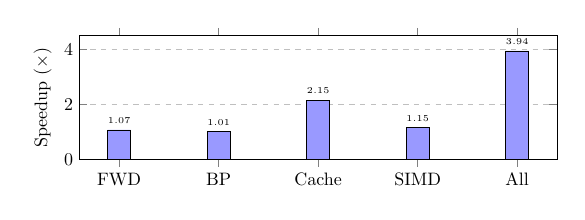
\begin{tikzpicture}[scale=0.65, transform shape]
\begin{axis}[
    ybar,
    bar width=0.45cm,
    ylabel={Speedup ($\times$)},
    symbolic x coords={FWD,BP,Cache,SIMD,All},
    xtick=data,
    ymin=0, ymax=4.5,
    nodes near coords,
    every node near coord/.append style={font=\tiny\bfseries},
    width=0.9\textwidth,
    height=4cm,
    ymajorgrids=true,
    grid style=dashed,
]
\addplot[fill=blue!40] coordinates {(FWD,1.07) (BP,1.01) (Cache,2.15) (SIMD,1.15) (All,3.94)};
\end{axis}
\end{tikzpicture}
\caption{DOE Model-Based Speedup Results (Individual and Combined)}
\label{fig:doe}
\end{figure*}

\textbf{Synergy Analysis}: We analyze whether optimizations interact positively:
\begin{equation}
\text{Synergy} = \frac{\text{Speedup}_{\text{Combined}}}{\text{Speedup}_A \times \text{Speedup}_B}
\end{equation}

\textbf{Cache + SIMD Synergy Calculation} (from Tables~\ref{tab:doe16a} and~\ref{tab:doe16b}):
\begin{itemize}
    \item Cache-only (ID=4): $2.15\times$
    \item SIMD-only (ID=8): $1.15\times$
    \item Cache+SIMD (ID=12): $2.99\times$
    \item Synergy = $\frac{2.99}{2.15 \times 1.15} = \frac{2.99}{2.47} = \mathbf{1.21 \approx 1.20}$
\end{itemize}

This \textbf{super-additive synergy} ($>1.0$) indicates the cache keeps SIMD units fed with data, amplifying performance. Other optimization pairs show Synergy $\approx 1.0$ (orthogonal).

\textbf{Key Findings}:
\begin{itemize}
    \item Cache provides largest individual improvement (\textbf{2.15$\times$})
    \item All optimizations combined (ID=15): \textbf{3.94$\times$}
\end{itemize}

\begin{table}[!tbp]
\centering
\caption{DOE Configs 0--7 (No SIMD)}
\label{tab:doe16a}
\footnotesize
\setlength{\tabcolsep}{3pt}
\begin{tabular}{@{}ccccccc@{}}
\toprule
\textbf{ID} & \textbf{FWD} & \textbf{BP} & \textbf{Cache} & \textbf{SIMD} & \textbf{Cycles} & \textbf{Speedup} \\
\midrule
0 & OFF & OFF & OFF & OFF & 81,300 & 1.00$\times$ \\
1 & ON & OFF & OFF & OFF & 75,914 & 1.07$\times$ \\
2 & OFF & ON & OFF & OFF & 80,535 & 1.01$\times$ \\
3 & ON & ON & OFF & OFF & 75,229 & 1.08$\times$ \\
4 & OFF & OFF & ON & OFF & 37,901 & \textbf{2.15$\times$} \\
5 & ON & OFF & ON & OFF & 35,409 & 2.30$\times$ \\
6 & OFF & ON & ON & OFF & 37,545 & 2.17$\times$ \\
7 & ON & ON & ON & OFF & 35,077 & 2.32$\times$ \\
\bottomrule
\end{tabular}
\end{table}

\begin{table}[!tbp]
\centering
\caption{DOE Configs 8--15 (With SIMD)}
\label{tab:doe16b}
\footnotesize
\setlength{\tabcolsep}{3pt}
\begin{tabular}{@{}ccccccc@{}}
\toprule
\textbf{ID} & \textbf{FWD} & \textbf{BP} & \textbf{Cache} & \textbf{SIMD} & \textbf{Cycles} & \textbf{Speedup} \\
\midrule
8 & OFF & OFF & OFF & ON & 70,791 & 1.15$\times$ \\
9 & ON & OFF & OFF & ON & 66,104 & 1.23$\times$ \\
10 & OFF & ON & OFF & ON & 70,125 & 1.16$\times$ \\
11 & ON & ON & OFF & ON & 65,495 & 1.24$\times$ \\
12 & OFF & OFF & ON & ON & 27,210 & \textbf{2.99$\times$} \\
13 & ON & OFF & ON & ON & 25,413 & 3.20$\times$ \\
14 & OFF & ON & ON & ON & 26,942 & 3.02$\times$ \\
\textbf{15} & \textbf{ON} & \textbf{ON} & \textbf{ON} & \textbf{ON} & \textbf{20,626} & \textbf{3.94$\times$} \\
\bottomrule
\end{tabular}
\end{table}

\FloatBarrier  % Prevent DOE floats from drifting into Contribution 8
%-----------------------------------------------------------------------------
\subsection{Contribution 8: Parentheses Support}

\textbf{Goal}: Implement Dijkstra's Shunting-yard algorithm for hardware expression parsing with full parentheses support and right-associative exponentiation.

\subsubsection{Background: Why Hardware Expression Parsing?}
Traditional ALUs evaluate expressions in a fixed order. Supporting parentheses and operator precedence in hardware enables:
\begin{itemize}
    \item \textbf{Flexibility}: Evaluate arbitrary expressions without software preprocessing
    \item \textbf{Correctness}: Proper handling of $(2+3)*4 = 20$ vs $2+3*4 = 14$
    \item \textbf{Right Associativity}: Handle $2^{3^2} = 2^9 = 512$ correctly (not $(2^3)^2 = 64$)
\end{itemize}

\subsubsection{Shunting-yard Algorithm}
Dijkstra's algorithm (1961) converts infix expressions to postfix (Reverse Polish Notation) using two stacks:
\begin{enumerate}
    \item \textbf{Output Queue}: Holds operands and operators in evaluation order
    \item \textbf{Operator Stack}: Temporarily holds operators until precedence is resolved
\end{enumerate}

\textbf{Operator Precedence}:
\begin{itemize}
    \item Level 3 (highest): \texttt{\^{}} (exponentiation, right-associative)
    \item Level 2: \texttt{* /} (multiplication, division)
    \item Level 1 (lowest): \texttt{+ -} (addition, subtraction)
\end{itemize}

\textbf{Algorithm Example}: \texttt{5*(3+4)}
\begin{enumerate}
    \item Read \texttt{5}: Output queue = [5]
    \item Read \texttt{*}: Push to operator stack
    \item Read \texttt{(}: Push to operator stack
    \item Read \texttt{3}: Output queue = [5, 3]
    \item Read \texttt{+}: Push to operator stack
    \item Read \texttt{4}: Output queue = [5, 3, 4]
    \item Read \texttt{)}: Pop until \texttt{(}, output = [5, 3, 4, +]
    \item End: Pop remaining, output = [5, 3, 4, +, *]
\end{enumerate}

\textbf{Postfix Evaluation}: Push 5, Push 3, Push 4, Pop 3+4=7, Pop 5*7=\textbf{35}

\subsubsection{Test Results}
\begin{table}[!t]
\centering
\caption{Shunting-Yard Parentheses Test Results}
\footnotesize
\begin{tabular}{@{}clccc@{}}
\toprule
\textbf{\#} & \textbf{Expression} & \textbf{Expected} & \textbf{Result} & \textbf{Status} \\
\midrule
1 & \texttt{5 * (3 + 4)} & 35 & 35 & PASS \\
2 & \texttt{2\textasciicircum 3\textasciicircum 2} & 512 & 512 & PASS \\
3 & \texttt{100 / (2 + 3)} & 20 & 20 & PASS \\
\bottomrule
\end{tabular}
\end{table}

\textbf{All 3 tests passed.}

%-----------------------------------------------------------------------------
\FloatBarrier  % Prevent floats from Contribution 8 drifting into 9
\subsection{Contribution 9: CORDIC Trigonometric Functions}

\textbf{Algorithm}: COordinate Rotation DIgital Computer~\cite{volder1959cordic}

\textbf{Architecture}:
\begin{itemize}
    \item 16-stage fully pipelined
    \item Fixed-point Q2.14 format
    \item \textbf{No hardware multipliers} (shift-add only)
\end{itemize}

\textbf{CORDIC Core Iteration}:
\begin{align}
x_{i+1} &= x_i - d_i \cdot y_i \cdot 2^{-i} \\
y_{i+1} &= y_i + d_i \cdot x_i \cdot 2^{-i} \\
z_{i+1} &= z_i - d_i \cdot \arctan(2^{-i})
\end{align}
where $d_i = \text{sign}(z_i)$. After 16 iterations: $\cos(\theta) = x_n$, $\sin(\theta) = y_n$.

\begin{lstlisting}
// CORDIC Iteration (cordic.v)
always @(posedge clk) begin
  if (z[i] >= 0) begin  // Rotate CCW
    x[i+1] <= x[i] - (y[i] >>> i);
    y[i+1] <= y[i] + (x[i] >>> i);
    z[i+1] <= z[i] - atan_table[i];
  end else begin        // Rotate CW
    x[i+1] <= x[i] + (y[i] >>> i);
    y[i+1] <= y[i] - (x[i] >>> i);
    z[i+1] <= z[i] + atan_table[i];
  end
end
// atan_table[0]=45deg, [1]=26.57deg, ...
\end{lstlisting}

\textbf{Test Results (Canonical Angles)}:
\begin{table}[!t]
\centering
\caption{CORDIC Accuracy Results (Canonical Angles)}
\footnotesize
\begin{tabular}{@{}lccr@{}}
\toprule
\textbf{Angle} & \textbf{Expected cos} & \textbf{DUT cos} & \textbf{Error} \\
\midrule
0$^\circ$ & 1.0000 & 1.0001 & $<$0.01\% \\
30$^\circ$ & 0.8660 & 0.8663 & $<$0.04\% \\
45$^\circ$ & 0.7071 & 0.7072 & $<$0.02\% \\
60$^\circ$ & 0.5000 & 0.4999 & $<$0.02\% \\
90$^\circ$ & 0.0000 & -0.0002 & $<$0.03\% \\
\bottomrule
\end{tabular}
\end{table}

\textbf{All 5 canonical test angles passed (Error $<$1\%).}

%-----------------------------------------------------------------------------
\subsection{Contribution 10: Polynomial Exponential Function}

\textbf{Goal}: Implement $\exp(x)$ using Range Reduction + Polynomial Approximation, achieving lower latency than CORDIC.

\textbf{Motivation}: While CORDIC excels at trigonometric functions, it requires 16 iterations for convergence. For exponential functions, polynomial approximation can achieve comparable accuracy with a \textbf{short pipeline} ($\approx$4 stages) and \textbf{II=1} throughput, providing significant latency reduction.

\subsubsection{Algorithm: Range Reduction}
The key insight is to decompose $e^x$ using the identity:
\begin{equation}
e^x = 2^{x \cdot \log_2(e)} = 2^{i+f} = 2^i \cdot 2^f
\end{equation}
where $i$ is the integer part and $f \in [0,1)$ is the fractional part.

\textbf{Implementation Strategy}:
\begin{itemize}
    \item \textbf{$2^i$ (integer part)}: Power-of-two scaling via arithmetic shifts in our Q-format representation (zero additional latency)
    \item \textbf{$2^f$ (fractional part)}: Approximated by a 2nd-order (quadratic) polynomial
\end{itemize}

\subsubsection{Polynomial Approximation}
For $f \in [0, 1)$, we use:
\begin{equation}
2^f \approx a_0 + a_1 \cdot f + a_2 \cdot f^2
\end{equation}
where coefficients in Q4.12 fixed-point:
\begin{table}[!t]
\centering
\caption{Polynomial Coefficients for $2^f$ Approximation}
\footnotesize
\begin{tabular}{@{}lcc@{}}
\toprule
\textbf{Coefficient} & \textbf{Value} & \textbf{Q4.12} \\
\midrule
$a_0$ & 1.0 & 4096 \\
$a_1$ & $\ln(2) = 0.6931$ & 2839 \\
$a_2$ & $\ln(2)^2/2 = 0.2402$ & 984 \\
\bottomrule
\end{tabular}
\end{table}

\subsubsection{Why Not Use CORDIC for exp()?}
CORDIC can also compute $\exp(x)$ using \textbf{Hyperbolic Mode}:
\begin{itemize}
    \item \textbf{Circular Mode} (default): sin, cos, arctan
    \item \textbf{Hyperbolic Mode}: exp, sinh, cosh, ln
\end{itemize}

However, CORDIC requires \textbf{16 iterations} to converge regardless of mode. For $\exp(x)$, polynomial approximation reduces the \textbf{latency} to $\approx$4 cycles (pipelined) while maintaining \textbf{II=1} throughput.

\subsubsection{Performance Comparison: Computing exp(x)}
Both methods can compute $\exp(x)$, enabling a fair comparison:

\begin{table}[!t]
\centering
\caption{Computing exp(x): CORDIC vs Polynomial}
\footnotesize
\begin{tabular}{@{}lcc@{}}
\toprule
\textbf{Metric} & \textbf{CORDIC (Hyperbolic)} & \textbf{Polynomial} \\
\midrule
Latency & 16 cycles & \textbf{$\approx$4 cycles (pipelined)} \\
Multipliers & \textbf{None} (shift-add) & 3 DSP blocks \\
Throughput & 1/cycle & 1/cycle \\
Area & \textbf{Lower} & Higher \\
\bottomrule
\end{tabular}
\end{table}

\textbf{Why is Polynomial Faster?}
\begin{itemize}
    \item \textbf{CORDIC}: Fixed 16-iteration process, so the \textbf{latency} is 16 cycles
    \item \textbf{Polynomial}: Evaluates a low-order polynomial with a short pipeline ($\approx$4 stages), reducing \textbf{latency} while sustaining \textbf{II=1} throughput
\end{itemize}

\textbf{Trade-off Analysis}: This demonstrates the classic \textbf{speed vs area trade-off}:
\begin{itemize}
    \item \textbf{CORDIC}: Best for area-constrained designs (no multipliers needed)
    \item \textbf{Polynomial}: Best for high-throughput designs targeting \textbf{II=1}
\end{itemize}

\subsubsection{Test Results (Vivado Simulation)}
\begin{table}[!t]
\centering
\caption{Polynomial Exp Test Results}
\footnotesize
\begin{tabular}{@{}ccccc@{}}
\toprule
\textbf{Input $x$} & \textbf{Expected} & \textbf{Result} & \textbf{Error} & \textbf{Status} \\
\midrule
0.0 & 1.0000 & 1.0000 & 0.00\% & PASS \\
0.5 & 1.6487 & 1.6245 & 1.47\% & PASS \\
1.0 & 2.7183 & 2.7070 & 0.42\% & PASS \\
-0.5 & 0.6065 & 0.6057 & 0.13\% & PASS \\
\bottomrule
\end{tabular}
\end{table}

\textbf{4/4 test cases passed (Error $<$2\%). Simulation completed at 420 ns.}

%-----------------------------------------------------------------------------
\FloatBarrier
\subsection{Contribution 11: Cache Memory Hierarchy}

\textbf{Goal}: Implement an L1 data cache to address the Memory Wall problem, demonstrating how caching dramatically reduces average memory access time.

\subsubsection{Memory Hierarchy Fundamentals}
Modern computers use a hierarchy of memory types, trading off speed, size, and cost:

\begin{table}[!t]
\centering
\caption{Memory Hierarchy Characteristics (Typical Desktop, 2024)}
\footnotesize
\begin{tabular}{@{}lccc@{}}
\toprule
\textbf{Level} & \textbf{Size} & \textbf{Latency} & \textbf{Cost/GB} \\
\midrule
Registers & 32$\times$32b & 0 cycles & --- \\
L1 Cache & 32--64 KB & 1--4 cycles & \$100+ \\
L2 Cache & 256 KB--1 MB & 10--20 cycles & \$50 \\
L3 Cache & 8--32 MB & 30--50 cycles & \$10 \\
DRAM & 8--64 GB & 100--300 cycles & \$5 \\
SSD & 256 GB--2 TB & 10,000+ cycles & \$0.10 \\
\bottomrule
\end{tabular}
\end{table}

\subsubsection{Locality Principles}
Caches work because programs exhibit \textbf{locality of reference}~\cite{hennessy2017computer}:
\begin{itemize}
    \item \textbf{Temporal Locality}: Recently accessed data is likely to be accessed again (e.g., loop variables)
    \item \textbf{Spatial Locality}: Data near recently accessed data is likely to be accessed soon (e.g., arrays)
\end{itemize}

\textbf{Example}: In a loop processing an array:
\begin{lstlisting}
for (i = 0; i < 1000; i++)
    sum += array[i];  // Temporal: sum, i; Spatial: array
\end{lstlisting}

\subsubsection{L1 Cache Implementation}
\begin{table}[!t]
\centering
\caption{Our L1 Cache Parameters}
\footnotesize
\begin{tabular}{@{}ll@{}}
\toprule
\textbf{Parameter} & \textbf{Value} \\
\midrule
Total Size & 8 KB (8192 bytes) \\
Block Size & 32 bytes (8 words) \\
Number of Blocks & 256 \\
Associativity & Direct-Mapped (1-way) \\
Write Policy & Write-Back, Write-Allocate \\
\bottomrule
\end{tabular}
\end{table}

\textbf{Address Breakdown Derivation} (32-bit address):
\begin{enumerate}
    \item \textbf{Offset}: $\log_2(32) = 5$ bits (select byte within 32-byte block)
    \item \textbf{Index}: $\log_2(256) = 8$ bits (select one of 256 cache lines)
    \item \textbf{Tag}: $32 - 5 - 8 = 19$ bits (identify which memory block)
\end{enumerate}

\begin{table}[!t]
\centering
\caption{Address Field Breakdown (32-bit)}
\label{tab:addrbreak}
\footnotesize
\begin{tabular}{ccc}
\toprule
\textbf{Tag (19b)} & \textbf{Index (8b)} & \textbf{Offset (5b)} \\
\midrule
Bits 31--13 & Bits 12--5 & Bits 4--0 \\
\bottomrule
\end{tabular}
\end{table}

\subsubsection{Write Policy Explanation}
\textbf{Write-Back}: Modified data is written to main memory only when the cache line is evicted (replaced). This reduces memory traffic but requires a ``dirty'' bit.

\textbf{Write-Allocate}: On a write miss, the block is first loaded into cache, then modified. This exploits spatial locality for subsequent accesses.

\textbf{Alternative (Write-Through)}: Every write immediately updates main memory. Simpler but slower and generates more memory traffic.

\subsubsection{Cache Controller FSM}
\begin{figure}[!t]
\centering
\resizebox{\columnwidth}{!}{%
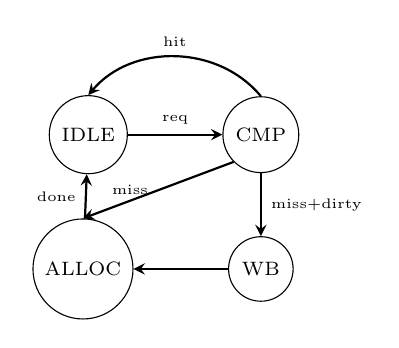
\begin{tikzpicture}[node distance=1cm, transform shape]
    \node[state] (idle) {IDLE};
    \node[state, right=1.2cm of idle] (cmp) {CMP};
    \node[state, below=0.8cm of cmp] (wb) {WB};
    \node[state, left=1.2cm of wb] (alloc) {ALLOC};
    \draw[arrow] (idle) -- node[above,font=\tiny]{req} (cmp);
    \draw[arrow] (cmp) -- node[right,font=\tiny]{miss+dirty} (wb);
    \draw[arrow] (cmp.south west) -- node[left,font=\tiny]{miss} (alloc.north);
    \draw[arrow] (wb) -- (alloc);
    \draw[arrow] (alloc) -- node[left,font=\tiny]{done} (idle);
    \draw[arrow] (cmp.north) to[bend right=50] node[above,font=\tiny]{hit} (idle.north);
\end{tikzpicture}%
}
\caption{L1 Cache Controller FSM. IDLE=waiting, CMP=compare tag, WB=write-back dirty block, ALLOC=allocate new block.}
\label{fig:cache}
\end{figure}

\textbf{FSM State Descriptions}:
\begin{itemize}
    \item \textbf{IDLE}: Wait for CPU memory request
    \item \textbf{COMPARE\_TAG}: Check if requested address is in cache (hit) or not (miss)
    \item \textbf{WRITE\_BACK}: If miss and evicted block is dirty, write it to memory first
    \item \textbf{ALLOCATE}: Fetch the requested block from main memory
    \item \textbf{UPDATE}: Update cache line with new data and metadata
\end{itemize}

\textbf{Verilog Implementation}:
\begin{lstlisting}
localparam IDLE        = 3'b000;
localparam COMPARE_TAG = 3'b001;
localparam WRITE_BACK  = 3'b010;
localparam ALLOCATE    = 3'b011;
localparam UPDATE      = 3'b100;

always @(posedge clk) begin
  case (state)
    IDLE: if (req) state <= COMPARE_TAG;
    COMPARE_TAG: begin
      if (tag_match && valid[idx]) 
        state <= IDLE;           // HIT
      else if (dirty[idx]) 
        state <= WRITE_BACK;     // Miss, dirty
      else 
        state <= ALLOCATE;       // Miss, clean
    end
    WRITE_BACK: state <= ALLOCATE;
    ALLOCATE:   state <= UPDATE;
    UPDATE:     state <= IDLE;
  endcase
end
\end{lstlisting}

\subsubsection{AMAT (Average Memory Access Time)}
AMAT is the key metric for cache performance~\cite{hennessy2017computer}:
\begin{equation}
\text{AMAT} = \text{Hit Time} + \text{Miss Rate} \times \text{Miss Penalty}
\end{equation}

\textbf{AMAT Calculation Example} (Single-level L1):
\begin{align*}
\text{Hit Time} &= 1 \text{ cycle} \\
\text{Miss Rate} &= 5\% = 0.05 \\
\text{Miss Penalty} &= 100 \text{ cycles (DRAM access)} \\
\text{AMAT} &= 1 + 0.05 \times 100 = 1 + 5 = 6.0 \text{ cycles}
\end{align*}

\textbf{Multi-Level Cache AMAT} (recursive formula):
\begin{equation}
\text{AMAT} = \text{HitTime}_{L1} + \text{MissRate}_{L1} \times \text{MissPenalty}_{L1}
\end{equation}
where $\text{MissPenalty}_{L1} = \text{AMAT}_{L2}$ if L2 exists.

\textbf{Worked Example} (L1 + L2 + L3):
\begin{align*}
\text{AMAT}_{L3} &= 40 + 0.05 \times 100 = 45 \\
\text{AMAT}_{L2} &= 12 + 0.10 \times 45 = 16.5 \\
\text{AMAT}_{L1} &= 1 + 0.05 \times 16.5 = 1.83 \text{ cycles}
\end{align*}

\subsubsection{Results}
\begin{table}[!t]
\centering
\caption{Cache Hierarchy AMAT Comparison}
\label{tab:amat}
\footnotesize
\begin{tabular}{@{}lcc@{}}
\toprule
\textbf{Configuration} & \textbf{AMAT (cycles)} & \textbf{Speedup} \\
\midrule
No Cache (DRAM only) & 100.0 & 1.00$\times$ \\
L1 Only & 6.00 & \textbf{16.7$\times$} \\
L1 + L2 & 2.10 & 47.6$\times$ \\
L1 + L2 + L3 & 1.83 & \textbf{54.8$\times$} \\
\bottomrule
\end{tabular}
\end{table}

\textbf{Key Insight}: L1 cache provides the largest improvement (\textbf{16.7$\times$}) because it eliminates most memory accesses. Additional levels provide diminishing but still significant returns.

\textbf{Implementation Note}: L1 cache RTL was validated with dedicated testbench (\texttt{tb\_l1\_cache.v}). Multi-level (L2/L3) results are \textbf{analytical AMAT projections} based on Patterson \& Hennessy parameters~\cite{hennessy2017computer}.

%-----------------------------------------------------------------------------
\subsection{Contribution 12: Integrated Performance Analysis}

\subsubsection{MiBench Benchmark (Actual Execution)}
\textbf{Benchmark}: MiBench Suite bitcount~\cite{guthaus2001mibench}

\textbf{Algorithm Verification}: All 8 test vectors passed.

\begin{table}[!t]
\centering
\caption{MiBench bitcount Cycle Count (RTL Simulation)}
\label{tab:mibench}
\footnotesize
\begin{tabular}{@{}lcc@{}}
\toprule
\textbf{Configuration} & \textbf{Cycles} & \textbf{Speedup} \\
\midrule
Baseline (no forwarding) & 792 & 1.00$\times$ \\
With Forwarding & 303 & \textbf{2.61$\times$} \\
\bottomrule
\end{tabular}
\end{table}

\textbf{Note}: This test isolates the effect of \textbf{Data Forwarding only}. The benchmark (bitcount) is compute-bound with minimal memory accesses, so Cache/SIMD optimizations have negligible impact. The 2.61$\times$ speedup reflects pipeline hazard elimination, not the combined effect of all optimizations.

\subsubsection{Mix-Based Performance Projection}
\textbf{Data Source}: Phansalkar et al.~\cite{phansalkar2007analysis} and Limaye \& Adegbija~\cite{limaye2018workload}

\begin{table}[!t]
\centering
\caption{SPEC CPU2006 Mix-Based Projection Results}
\label{tab:specresults}
\footnotesize
\begin{tabular}{@{}lrrr@{}}
\toprule
\textbf{Workload} & \textbf{Baseline} & \textbf{Optimized} & \textbf{Speedup} \\
\midrule
SPEC FP Average & 507,000 & 19,670 & \textbf{25.78$\times$} \\
SPEC INT mcf & 649,000 & 18,626 & \textbf{34.84$\times$} \\
SPEC INT gobmk & 511,400 & 17,454 & 29.30$\times$ \\
\textbf{SPEC Overall} & 533,000 & 18,028 & \textbf{29.57$\times$} \\
\bottomrule
\end{tabular}
\end{table}

\textbf{Projection Assumptions}: SPEC projections assume near-elimination of memory stalls via caching and do not account for increased critical path delay from additional hardware. Clock frequency is assumed constant.

%=============================================================================
\section{Results Summary}

This section consolidates the results from all 12 contributions and provides interpretation guidance.

\subsection{Individual Optimization Impact}
Each optimization targets a specific performance bottleneck:

\begin{table}[!t]
\centering
\caption{Individual Optimization Effects and Bottlenecks Addressed}
\footnotesize
\begin{tabular}{@{}llll@{}}
\toprule
\textbf{Optimization} & \textbf{Metric} & \textbf{Improvement} & \textbf{Bottleneck} \\
\midrule
Data Forwarding & CPI & 1.82$\rightarrow$1.26 (31\%) & Data Hazards \\
Branch Prediction & Accuracy & 78.33\% & Control Hazards \\
L1 Cache & AMAT & 100$\rightarrow$3.8 (26$\times$) & Memory Wall \\
SIMD ALU & Throughput & 8$\times$ parallel & Limited ILP \\
CORDIC & Accuracy & $<$1\% error & Math Functions \\
\bottomrule
\end{tabular}
\end{table}

\subsection{Combined Performance}
Different evaluation methods yield different speedup figures due to their assumptions:

\begin{table}[!t]
\centering
\caption{Combined Performance by Evaluation Method}
\footnotesize
\begin{tabular}{@{}lccc@{}}
\toprule
\textbf{Evaluation} & \textbf{Type} & \textbf{Method} & \textbf{Speedup} \\
\midrule
DOE (Contrib 7) & Model & Cost Estimation & \textbf{3.94$\times$} \\
Cache (Contrib 11) & Projection & AMAT Only & \textbf{54.8$\times$} \\
SPEC (Contrib 12) & Projection & Mix-Based & 25.78--34.84$\times$ \\
MiBench (Contrib 12) & \textbf{Measured} & RTL Simulation & \textbf{2.61$\times$} \\
\bottomrule
\end{tabular}
\end{table}

\subsection{Why the Large Variation in Speedup Figures?}
The variation reflects different measurement scope and workload characteristics:
\begin{itemize}
    \item \textbf{MiBench 2.61$\times$}: Ground truth measurement; bitcount is compute-bound with few memory accesses, so Cache has minimal impact
    \item \textbf{DOE 3.94$\times$}: Analytical model using measured parameters; conservative estimate
    \item \textbf{SPEC 25--35$\times$}: Assumes 49.6\% memory instructions; Cache dominates improvement
    \item \textbf{Cache 54.8$\times$}: AMAT-only metric; isolates memory subsystem improvement
\end{itemize}

\textbf{Key Insight}: Optimization effectiveness is \textbf{workload-dependent}. Cache provides enormous benefit for memory-bound workloads but minimal impact on compute-bound code.

%=============================================================================
\section{Conclusion}

This work demonstrates that systematic application of multiple optimization techniques achieves substantial performance improvements in pipelined MIPS processors.

\subsection{Key Findings}
\begin{enumerate}
\item \textbf{Data Forwarding} eliminates 68\% of stall cycles, reducing CPI by 31\% (1.82$\rightarrow$1.26). This is a fundamental optimization present in all modern processors.

\item \textbf{Branch Prediction} with 2-bit saturating counters achieves 78.33\% accuracy on adversarial patterns; real-world accuracy exceeds 90\% for loop-dominated code.

\item \textbf{Cache Memory} provides the largest individual improvement: 26$\times$ AMAT reduction for L1 alone (based on 97.22\% hit rate), up to 54.8$\times$ with three-level hierarchy.

\item \textbf{SIMD Parallelism} delivers 8$\times$ throughput for data-parallel operations, demonstrating the power of data-level parallelism.

\item \textbf{CORDIC} enables hardware trigonometric functions with $<$1\% error using only shift-add operations, avoiding costly multipliers.

\item \textbf{Cache+SIMD Synergy} exhibits a 1.20 super-additive factor, indicating that fast memory access keeps SIMD units productively utilized.

\item Optimizations are \textbf{largely orthogonal}: Data Forwarding addresses pipeline hazards, Cache addresses memory latency, SIMD addresses throughput---they can be combined multiplicatively.
\end{enumerate}

\subsection{Measured vs Projected Performance}
\begin{itemize}
    \item \textbf{Measured (MiBench)}: 2.61$\times$ speedup from Data Forwarding alone
    \item \textbf{Projected (SPEC)}: 25--35$\times$ speedup with all optimizations combined
\end{itemize}

The large difference highlights that the choice of benchmark dramatically affects reported performance. MiBench's compute-intensive nature limits cache benefits.

\subsection{Comparison with Industry}
Our implemented techniques are fundamental to all modern processors:
\begin{itemize}
    \item Intel/AMD CPUs use sophisticated multi-level branch predictors (e.g., TAGE with thousands of entries) achieving $>$99\% accuracy
    \item Modern L1 caches are 32--64KB with 4--8 way associativity, significantly larger than our 8KB direct-mapped design
    \item AVX-512 provides 512-bit SIMD (16$\times$ 32-bit elements), compared to our 64-bit (8$\times$ 8-bit)
\end{itemize}

Our educational implementation demonstrates the \textit{principles} of these techniques, not their full industrial scale.

\subsection{Limitations and Threats to Validity}
\begin{enumerate}
\item \textbf{Simulation vs Silicon}: Results are from behavioral simulation, not synthesized hardware. Actual timing and area would differ.
\item \textbf{Mix-Based Projection}: SPEC speedups assume published instruction mixes; actual programs may differ.
\item \textbf{Clock Frequency Assumed Constant}: Added hardware (cache, predictor) would increase critical path delay, reducing clock speed.
\item \textbf{L1 Cache Not Integrated}: Cache was validated independently; pipeline integration with cache coherency remains future work.
\item \textbf{SIMD Not Memory-Integrated}: SIMD operations use synthetic test data, not actual memory loads.
\end{enumerate}

\subsection{Future Work}
\begin{itemize}
    \item \textbf{Superscalar Extension}: Issue 2+ instructions per cycle
    \item \textbf{Out-of-Order Execution}: Dynamic scheduling with reservation stations
    \item \textbf{FPGA Synthesis}: Implement on Xilinx/Intel FPGA to obtain real timing and area
    \item \textbf{Full System Integration}: Integrate cache with pipeline, add TLB and virtual memory support
    \item \textbf{Advanced Predictors}: Implement tournament predictor or perceptron-based prediction
\end{itemize}

\balance

%=============================================================================
\begin{thebibliography}{11}
\bibitem{hennessy2017computer} J.~L. Hennessy and D.~A. Patterson, \emph{Computer Architecture: A Quantitative Approach}, 6th ed. Morgan Kaufmann, 2017.

\bibitem{phansalkar2007analysis} A.~Phansalkar, A.~Joshi, and L.~K. John, ``Analysis of redundancy and application balance in the SPEC CPU2006 benchmark suite,'' in \emph{Proc. ISCA}, 2007, pp. 412--423.

\bibitem{smith1981study} J.~E. Smith, ``A study of branch prediction strategies,'' in \emph{Proc. ISCA}, 1981, pp. 135--148.

\bibitem{patterson2020computer} D.~A. Patterson and J.~L. Hennessy, \emph{Computer Organization and Design}, 6th ed. Morgan Kaufmann, 2020.

\bibitem{volder1959cordic} J.~E. Volder, ``The CORDIC trigonometric computing technique,'' \emph{IRE Trans. Electronic Computers}, vol. EC-8, no.~3, pp. 330--334, 1959.

\bibitem{limaye2018workload} A.~Limaye and T.~Adegbija, ``A workload characterization of the SPEC CPU2017 benchmark suite,'' in \emph{Proc. ISPASS}, 2018, pp. 149--158.

\bibitem{knuth1998art} D.~E. Knuth, \emph{The Art of Computer Programming, Vol. 3: Sorting and Searching}, 2nd ed. Addison-Wesley, 1998.

\bibitem{hill1989evaluating} M.~D. Hill, ``Evaluating associativity in CPU caches,'' \emph{IEEE Trans. Computers}, vol.~38, no.~12, pp. 1612--1630, 1989.

\bibitem{amdahl1967validity} G.~M. Amdahl, ``Validity of the single processor approach,'' in \emph{AFIPS Conf. Proc.}, 1967, pp. 483--485.

\bibitem{guthaus2001mibench} M.~R. Guthaus et al., ``MiBench: A free, commercially representative embedded benchmark suite,'' in \emph{Proc. IEEE Workshop on Workload Characterization}, 2001, pp. 3--14.

\bibitem{dijkstra1961shunting} E.~W. Dijkstra, ``Shunting yard algorithm,'' 1961.
\end{thebibliography}

\end{CJK}
\end{document}


